\section{Measuring the performance of the pipeline}\label{e2e}

Above results reflect the performance of the \ac{ASR} model alone. To get some insight about the quality of alignments produced by the whole pipeline, a simple web application was implemented that highlights the aligned parts of the transcript as the audio file is being played. This is very useful for an informal review, because the subjective quality of the alignments can be examined interactively. However, this method is not very systematic and infeasible for larger amounts of test data. To get a clearer sense of how well the pipeline performed, steps were taken to run large numbers of previously unseen samples through the pipeline and measure the quality of the alignments produced. This section describes how this was done.

\subsection{The quality of alignments}

Assessing the quality of alignments is not trivial because there is often no reference alignment to compare to. Even if there is one, assessing the quality of an alignment is somewhat subjective because there is a a massive number of theoretically possible alignments for each transcript. We can however derive a few objective criteria that make up a good alignment:

\begin{enumerate}
	\item The aligned partial transcripts should not overlap each other
	\item The alignments should neither start nor end within word boundaries
	\item The aligned partial transcripts should cover the as much of the original transcript as possible	
	\item The aligned partial transcripts should be at the correct position (i.e. they should cover the actually spoken text)
\end{enumerate}

The first criterion is enforced by changing the type of algorithm used for sequence alignment from a local to a global alignment algorithm. During the IP8 project, the \textit{Smith-Waterman} algorithm was used in the \ac{LSA} stage, which finds a local optimum for each transcript individually. This was replaced by the \textit{Needle-Wunsch} algorithm, which finds an optimal alignment for all partial transcrips at once. 

The second criterion is ensured by adjusting some of the alignments produced by \textit{Needle-Wunsch} so that they fall exactly on word boundaries.

The remaining two criteria can be quantified with the following metrics (note the corellation\footnote{positive correlation: higher is better, negative correlation: lower is better}):

\begin{table}[!htbp]
	\centering
	\begin{tabular}{|l|l|l|l|}
		\hline
		\thead{criterion} & \thead{metric} & \thead{symbol} & \thead{correlation} \\
		\hline
		1 & \makecell[l]{length of text in ground truth that is not aligned vs. total length of the ground truth} & $C$ & negative \\ 
		\hline		
		3 & \makecell[l]{average Levensthein similarity between the transcript\\and the text in the ground truth corresponding to its alignment} & $D$ & positive \\ 
		\hline				
	\end{tabular}
	\caption{Metrics to evaluate the quality of alignments}
	\label{LM_evaluation}
\end{table}

Because the first metric measures how much of the target transcript is covered by the alignments, it is somewhat similar to the Recall $R$. The second metric measures how well the produced results match up with the underlying parts of the transcript and is therefore similar to Precision $P$. Both metrics can therefore be reduced to the F-score, a single number usually used to evaluate classification results:

\[ 
F = 2\cdot \frac{P\cdot R}{P+R}
 \]

Figure \ref{example_alignment} shows an example of an alignment. The sentence was split into speech segments by \ac{VAD} which were then aligned with the whole sentence (ground truth). Some speech segments were misaligned, resulting in an overlap. Some of the transcriptions contain mistakes. Note that the Levensthein Similarity ($ls(s_1, s_2)$) measures the similarity of two strings $s_1$ and $s_2$ as the normalized edit distance and is calculated as follows:

\begin{equation}
	ls(s_1, s_2) = 1 - \frac{ed(s_1, s_2)}{max \left(len(s_1), len(s_2), len(s_3)\right)}
\end{equation}

For $t_1=\text{i see}, t_2=\text{i c}, t_3 = \text{sad the blind men}, t_4 = \text{to his blind daughter}$ The metrics can be calculated as follows:

\begin{equation}
C = \frac{len(\text{i see})}{len(\text{i see i see said the blind man to his deaf daughter})} = \frac{5}{51} = 0.098
\end{equation}

\begin{equation}
\begin{split}
O & = \frac{len(\text{i see})}{len(\text{i see}) + len(\text{i c}) + len(\text{sad the blind men}) + len(\text{to his deaf daughter})} \\
 & = \frac{5}{5 + 3 + 17 + 20} = 0.11
\end{split}
\end{equation}

\begin{equation}
\begin{split}
D & = \frac{ls(\text{i see}, t_1) + ls(\text{i see}, t_2) + ls(\text{said the blind man}, t_3) + ls(\text{to his deaf daughter}, t_4)}{4} \\
 & = \frac{1 + 0.4 + 0.88 + 1}{4} = 0.82
\end{split}
\end{equation}

\begin{figure}
	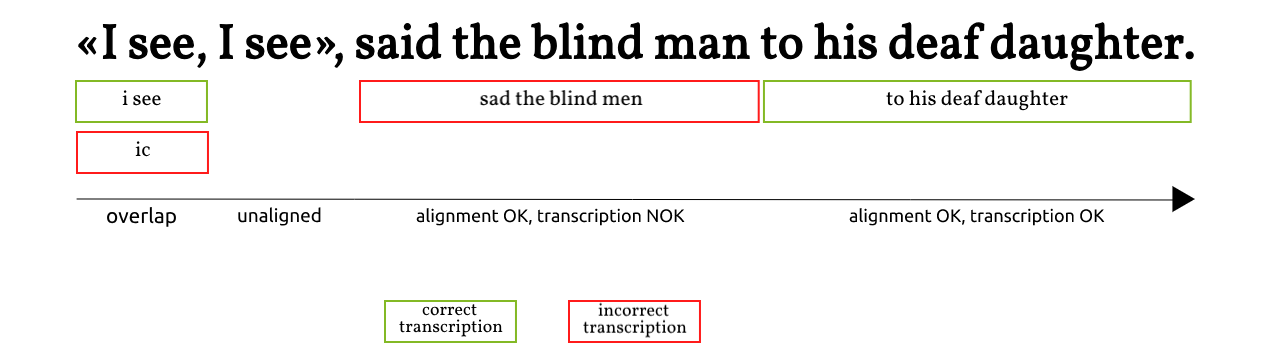
\includegraphics[width=\linewidth]{./img/example_alignment.png}
	\caption{Example for a partially correct alignment of parts of a sentence}
	\label{example_alignment}
\end{figure}

\subsection{Test and results}

The pipeline was evaluated using the model with the lowest average validation-\ac{LER}. For English, this was the model with dropouts. To prevent overfitting, training was stopped after x epochs (early stopping). The pre-trained \ac{DS} model was used as a reference model for comparison.

$P$, $R$ and $F$ were calculated for English and German by running each sample from the test set of the respective corpus through the pipeline.

\subsection{Pipeline performance using an \ac{ASR} model for a different language}

Due to an implementation error the samples from the German test set were run through the pipeline using an \ac{ASR} for English at some point in the testing phase. The error was corrected, but surprisingly enough, the transcripts produced were still accurate enough for alignment. Apparently, the Needle-Wunsch algorithm used in the global alignment stage only needs very little resemblance of the partial transcripts to the real transcripts in order produce alignments that are usable, although maybe a bit worse.